
%Here I need to go through and describe all of the things that are important for the discussion
%aim for 20 pages

%things to discuss include:
%- A general introduction to the standard model (probably no more than a page or two)
%- Electroweak physics
%- W decay
%- parton distribution functions (maybe with some thorough discussion on this) as well as renormalization and factorization scales

%- WWW production (do I actually want to discuss this at all here??)
%- Effective field theory and anomalous coupling measurements


%assuming these will be defined here
% Quartic Gauge Couplings (QGC) 
% Standard Model (SM)
% anomalous Quartic Gauge Couplings (aQGC)
% Parton Distribution Function (PDF)


\section{The Standard Model}

The Standard Model (SM) is a theory which describes all of the
observed matter and interactions in the universe, except for gravity.
It is built from a quantum field theory where the constituent particles
and interactions fit into a non-Abelian 
$\suthree\times\sutwo\times\uone$~gauge symmetry.
From these symmetries come the matter fermions, split 
into the quarks and leptons, and the force-carrying bosons
that mediate their interactions.
The \suthree~symmetry describes the theory of Quantum Chromodynamics (QCD)
which explains the interaction of the quarks via the gluons, the
gauge bosons that mediate the strong force.
The remaining $\sutwo\times\uone$~symmetry 
describes the Electroweak (EW) theory which explains
the interactions of the quarks and leptons via the 
electroweak gauge bosons that mediate
the electroweak force: $W$, $Z$, and $\gamma$ (i.e. the photon).
The EW theory is itself a unified description of the weak force,
involving the $W$ and $Z$, and the electromagnetic force, involving
just the photon.
The $W$ and $Z$ gauge bosons (as well as the quarks and leptons) receive
their non-zero masses through the process of electroweak symmetry
breaking (EWSB). The simplest form of EWSB
introduces an additional 'Higgs' field that
predicts a single new fundamental scalar boson. This boson is the
famous Higgs boson which was discovered recently at the 
LHC \cite{Aad20121,Chatrchyan:2012xdj}, thereby
confirming this last component of the SM.
%cite

All of the 
observed fundamental 
matter particles in the universe are described by the quark
and leptons of the SM. Their properties are listed 
in \tab\ref{tab:theory_fermions}. 
The particles can be distinguished
by their charges and masses.
The charges describe how (and if) the particles participate in
different interactions.
Those fermions with electric charge (all but the neutrinos) 
participate in the electromagnetic
interactions. The quarks have color charge (sometimes 
just called color), which allows them to 
participate in the QCD interactions. All fermions also participate in 
the weak interactions. The types of allowed weak interactions are determined
by a combination of the electric charge as well as the weak isospin
and weak hypercharge, described in \sec\ref{sec:theory_ew}.
%explain better
Since all of the particles are fermions, they all have a spin of 1/2.
The masses of the particles are not predicted by the theory, but 
are essential for understanding their stability and decay properties
as well as their kinematic behavior.
Each particle also has a corresponding anti-particle with the same mass but
whose electric charge has opposite sign. The neutrinos, with zero 
electric charge, could possibly be their own 
anti-particle (so-called Majorana fermions), but
this has yet to be confirmed.
The quarks and leptons can each be divided up into three ``generations'' 
composed of pairs
of particles with identical charges but whose masses increase with each generation.
The generations are labeled in \tab\ref{tab:theory_fermions}. 
Even though there are three 
generations in both the lepton and quark sectors, 
the quarks and leptons are not observed to interact directly, 
thus the quark and lepton generations should be thought of as separate.

\begin{table}[ht]
\centering
\small
\begin{tabular}{|lclc|c|c|}
\hline
                        & Generation & Name & Symbol  & Charge & Mass [MeV]\\
\hline
\hline
\multirow{6}{*}{Quarks}& \multirow{2}{*}{First}& Up & $u$   &  $~~2/3$    &  $2.3 ^{+0.7}_{-0.5}$    \\
                       & & Down & $d$  &  $-1/3$    &  $4.8^{+0.5}_{-0.3}$    \\
		       \cline{2-6} 
                       &\multirow{2}{*}{Second}& Charm & $c$   & $~~2/3$     & $1275 \pm 25$     \\
                       && Strange & $s$   & $-1/3$     & $95 \pm 5$     \\
		       \cline{2-6} 
                       &\multirow{2}{*}{Third}& Top & $t$   &  $~~2/3$    &  $173210 \pm 874$    \\
                       && Bottom & $b$   &  $-1/3$    & $4180 \pm 30$     \\
\hline
\hline
\multirow{6}{*}{Leptons}&\multirow{2}{*}{First} &Electron & $e$     &  -1    &  $0.510998928 \pm 0.000000011 $ \\
                        & & Electron Neutrino & $\nu_e$  & 0    &   $ < 0.002$    \\
		       \cline{2-6} 
                        &\multirow{2}{*}{Second} &Muon & $\mu$     &   -1   &   $105.6583715 \pm 0.0000035$   \\
                        & &Muon Neutrino & $\nu_{\mu}$  & 0   &  $ < 0.19$    \\
		       \cline{2-6} 
                        & \multirow{2}{*}{Third}&Tau & $\tau$     &   -1   &  $1776.86 \pm 0.12$    \\
                        & &Tau Neutrino & $\nu_{\tau}$  & 0    &  $< 18.2 $    \\
\hline
\end{tabular}
\label{tab:theory_fermions}
\caption{Summary of the electric charge and measured masses of the SM fermions. Mass measurements
are taken from the Particle Data Group \cite{PDG:2014} and 
are shown to the best precision available with their measured uncertainties.
Particles are also organized by their generation.
The bottom quark mass measurement is shown using the $\overline{\textrm{MS}}$ 
renormalization scheme.
The top quark mass uncertainty combines the reported statistical and 
systematic uncertainties 
in quadrature.
The limits on the electron neutrino and muon neutrino masses are 
set at a 90\% confidence level 
while the tau neutrino limits are set at a 95\% confidence level.}
\end{table}



The SM can be written down using a lagrangian of the form
\begin{equation}
\curlyl_{\textrm{SM}} = \curlyl_{\textrm{QCD}} + \curlyl_{\textrm{EW}} + \curlyl_{\textrm{EWSB}}
\label{eq:lagrangian_sm}
\end{equation}
which satisfies global and local gauge invariance.
From this, one can calculate all of the fundamental interactions of the SM.
As written, the SM lagrangian can be split up into separate terms describing the
QCD, EW, and EWSB behavior. 
The details of each term are described in more detail below.


\subsection{Quantum Chromodynamics}
The QCD term in the SM lagrangian can be written as
\begin{equation}
\begin{aligned}
\curlyl_{\textrm{QCD}} = &-\frac{1}{4}G^a_{\mu\nu} G_a^{\mu\nu} 
                         -g_s \Big( \overline{q} \gamma^{\mu} T_a q \Big) G_{\mu}^a \\
			 &+\overline{q}\Big( i\gamma^{\mu} \partial_{\mu} - m\Big) q
\end{aligned}
\label{eq:lagrangian_qcd}
\end{equation}
implied sum over three color fields $q_1$,$q_2$, $q_3$

$T_a$ are the generators of \suthree~, represented by the eight Gell-Mann matrices.
\begin{equation}
G_{\mu\nu}^a = \partial_{\mu} G^a_{\nu} - \partial_{\nu} G^a_{\mu} - g f_{abc} G_{\mu}^b G_{\nu}^c
\end{equation}

$G_{\mu}^a$ are the gluon fields

\begin{equation}
\Big[T_a,T_b\Big] = i f_{abc} T_c
\end{equation}

$f_{abc}$ are the structure constants which are antisymmetric

Sum over $a$

non-Abelian means self-interacting

color confinement. 
comes from anti-screening which is a direct result of the non-Abelian 
nature of QCD. ch1 and ch7.9


value of $g_s$ determined by number of quarks 
which results in non-perturbativity

\subsection{Parton Distribution Functions}
Parton Distribution Function (PDF)

Include valence quark rules

sea quarks

asymptotic freedom

\subsection{The Electroweak Theory}
\label{sec:theory_ew}
The electroweak (EW) 
theory of Glasgow, Weinberg, and 
Salam \cite{glashow:1961tr,Salam:1968rm,weinberg:1967tq}
is a renormalizable \cite{hooft1971renormalization,Hooft1971167}
non-Abelian gauge theory 
that successfully unifies the theories 
of the \uone~electromagnetism and \sutwo~weak interactions.
It incorporates the observed 
charge conjugation ($C$) 
and parity ($P$) violating V-A structure of the weak interactions
\cite{PhysRev.105.1413,Garwin:1957hc,PhysRev.106.1290}
while simultaneously preserving these symmetries for electromagnetism.
It explains the presence of the massive EW gauge bosons 
while maintaining gauge invariance
using spontaneous symmetry breaking
and includes the observed CP violating 
\cite{PhysRevLett.13.138} 
flavor mixing of the 
charged interactions in the quark sector via 
the Cabibbo-Kobayashi-Maskawa  (CKM)
matrix \cite{Cabibbo:1963yz,Kobayashi:1973fv}.

The EW term in the SM lagrangian can be written as
\begin{equation}
\begin{aligned}
\curlyl_{\textrm{EW}} = -\frac{1}{4}\textbf{W}_{\mu\nu} \cdot \textbf{W}^{\mu\nu} 
- \frac{1}{4} B_{\mu\nu} B^{\mu\nu}  +\overline{\psi}\gamma^{\mu}D_{\mu}\psi
\end{aligned}
\label{eq:lagrangian_ew}
\end{equation}
where the first two terms describe the kinetic energies and 
self-interactions of the EW gauge bosons
and the last term describes the fermion kinetic energies
and their interactions with the EW gauge bosons.
The kinetic energies are described by the field strength tensors
\begin{equation}
\label{eq:wfieldstrength}
\textbf{W}_{\mu\nu} = \partial_{\mu}\textbf{W}_{\nu} - \partial_{\nu}\textbf{W}_{\mu} - g \textbf{W}_{\mu}\times \textbf{W}_{\nu}
\end{equation}
and 
\begin{equation}
\label{eq:bfieldstrength}
B_{\mu\nu} = \partial_{\mu} B_{\nu} - \partial_{\nu} B_{\mu}
\end{equation}
The gauge fields, $\mathbf{W}_{\mu}$ and $B_{\mu}$, represent the 
massless EW gauge bosons before EWSB. They are four-vectors of the Lorentz group
and thus undergo Lorentz transformations as indicated by their Lorentz index, $\mu$.
The $\partial_{\mu}$ is the four-dimensional partial derivative of the Lorentz
group and the $\gamma^{\mu}$ are the Dirac matrices.
The EW covariant derivative, $D_{\mu}$, is
\begin{equation}
D_{\mu} =  i \partial_{\mu} - g \frac{1}{2} \boldsymbol{\tau} \cdot \textbf{W}_{\mu} - g' \frac{Y}{2} B_{\mu} 
\label{eq:ew_covariant_derivative}
\end{equation}
The coupling constants $g$ and $g'$ describe the strength of the interactions
of the fermions with the gauge boson fields before EWSB. 
The $\mathbf{W}_{\mu}$ describes two charged gauge bosons and 
a neutral gauge boson as an isotriplet of 
vector fields ($W_{\mu}^i$)
in \sutwo~with its generators being the famous Pauli matrices, $\boldsymbol{\tau}$.
The charged gauge bosons are represented by a superposition of the first
two components of the 
isotriplet, $W_{\mu}^{\pm}=\sqrt{\frac{1}{2}}\Big(W_{\mu}^1\mp i W_{\mu}^2\Big)$,
while the neutral gauge boson is represented 
by the third component, $W_{\mu}^3$.
The $B_{\mu}$ describes a single neutral gauge boson 
using a single vector field in \uone~with the generator $Y$, referred
to as the weak hypercharge.
By construction, the weak hypercharge is related to
the electric charge of \uone~
electromagnetism, $Q$, 
and the charge of the third component of weak \sutwo, $T^3$:
\begin{equation}
Q=T^3+Y/2
\label{eq:ewcharges}
\end{equation}
The fermion fields, $\psi$, (and their conjugates, $\overline{\psi}$)
can be split up into the 
left-handed fermion isospin doublets, $L$,  and right-handed
fermion isospin singlets, $R$, which is described in more detail later.
Putting it all together, we end up with
\begin{equation}
\begin{aligned}
\curlyl_{\textrm{EW}} = 
& -\frac{1}{4}\Big(\partial_{\mu}\textbf{W}_{\nu} - \partial_{\nu}\textbf{W}_{\mu} - g \textbf{W}_{\mu}\times \textbf{W}_{\nu}\Big) \cdot \Big(\partial^{\mu}\textbf{W}^{\nu} - \partial^{\nu}\textbf{W}^{\mu} - g \textbf{W}^{\mu}\times \textbf{W}^{\nu}\Big)  \\
& -\frac{1}{4}\Big(\partial_{\mu} B_{\nu} - \partial_{\nu} B_{\mu}\Big) 
\Big(\partial^{\mu} B^{\nu} - \partial^{\nu} B^{\mu}\Big)\\
&+\overline{L}\gamma^{\mu}\Big( i \partial_{\mu} - g \frac{1}{2} \boldsymbol{\tau} \cdot \textbf{W}_{\mu} - g' \frac{Y}{2} B_{\mu} \Big) L \\
&+ \overline{R} \gamma^{\mu} \Big( i \partial_{\mu} - g' \frac{Y}{2} B_{\mu} \Big) R
\end{aligned}
\label{eq:lagrangian_ew_expanded}
\end{equation}



The V-A structure of the weak interactions
results in the absence of charged weak interactions involving right-handed
fermions and left-handed anti-fermions.
This is captured
by assigning charges to the SM fermions 
as listed in \tab\ref{tab:ewcharges}
such that they satisfy \eqn\eqref{eq:ewcharges}.
The charges differ based on the helicity, or ``handedness'',
of the fermions.
This specification for the charges results in the 
left-handed fermion fields being treated as isospin doublets, $L$, 
which transform under \sutwo~for each lepton and quark generation:
\begin{equation}
L = 
\begin{pmatrix} e_L \\ \nu_{e,L} \end{pmatrix},
\begin{pmatrix} \mu_L \\ \nu_{\mu,L} \end{pmatrix},
\begin{pmatrix} \tau_L \\ \nu_{\tau,L} \end{pmatrix},
\begin{pmatrix} u_L \\ d_{L} \end{pmatrix},
\begin{pmatrix} c_L \\ s_{L} \end{pmatrix},
\begin{pmatrix} t_L \\ b_{L} \end{pmatrix}
\end{equation}
while the right-handed fermion fields are treated as isospin singlets, $R$, 
which only transform under \uone:
\begin{equation}
R = e_R,~\mu_R,,~\tau_R,~u_R,~d_R,~c_R,~s_R,~t_R,~b_R
\end{equation}
where each object is a Dirac field whose helicity is indicated by 
its subscript.
Note that the right-handed neutrinos are absent.
This comes from them having zero charge across 
the board in \tab\ref{tab:ewcharges}.
As a result, they do not participate in any of the SM interactions
and only exist hypothetically as so-called ``sterile'' neutrinos.
%refer to first observation of missing right-handed neutrinos?

\begin{table}[ht]
\centering
\begin{tabular}{llc|ccc}
  \multicolumn{3}{c|}{Particle} & $Q$ & $Y$ & $T^3$\\
\hline
\hline
\multirow{4}{*}{Quarks} & \multirow{2}{*}{Left-Handed}&  $u_L$   &  2/3  &1/3 & 1/2  \\
                       &                              &  $d_L$  & -1/3   &1/3& -1/2 \\
		       \cline{2-6}
                       &\multirow{2}{*}{Right-Handed}&  $u_R$   & 2/3  & 4/3 & 0 \\
                       &                             &  $d_R$  & -1/3   &-2/3& 0\\
\hline
\hline
\multirow{4}{*}{Leptons}&\multirow{2}{*}{Left-Handed} &$e_L$     & -1  & -1& 1/2\\
                        &                             & $\nu_{e,L}$  & 0 &-1&-1/2 \\
		       \cline{2-6}
                        &\multirow{2}{*}{Right-Handed} &$e_R$     & -1  & -2& 0\\
                        &                              & $\nu_{e,R}$  & 0 &0 &0 \\
\end{tabular}
\caption{The charges of the SM fermions. The charges are the same
for each generation, so only the first generation of quarks
and leptons are shown.  } %what about T?
\label{tab:ewcharges}
\end{table}

Using this specification of the fermion fields 
we can identify the interactions of the fermions with the 
charged $W$ boson.  Expanding the term 
\begin{equation}
-g \frac{1}{2} \overline{L}\gamma^{\mu}\boldsymbol{\tau} \cdot \textbf{W}_{\mu} L 
\end{equation}
from \eqn\eqref{eq:lagrangian_ew_expanded}
and keeping only those
terms where the charged $W$ and lepton fields are present gives
\begin{equation}
\begin{aligned}
%\overline{u'}_R W_{\mu}^+ d'_L +
%\overline{d'}_R W^-_{\mu} u'_L +
\frac{g}{\sqrt{2}}\gamma^{\mu}\Big( &
\overline{e}_R W_{\mu}^+ \nu_{e,L} +
\overline{\nu}_{e,R} W^-_{\mu} e_L \\&+
\overline{\mu}_R W_{\mu}^+ \nu_{\mu,L} +
\overline{\nu}_{\mu,R} W^-_{\mu} \mu_L \\&+
\overline{\tau}_R W_{\mu}^+ \nu_{\tau,L} +
\overline{\nu}_{\tau,R} W^-_{\mu} \tau_L \Big)
\end{aligned}
\label{eq:couplings_wleptons}
\end{equation}
which corresponds to the Feynman diagrams at the top
of \fig\ref{fig:feyn_wcoupling}. It is this
type of interaction that is responsible for the $W$ decay to leptons.
In the absence of quark flavor mixing, the interaction terms 
of the quark sector look similar:
\begin{equation}
\begin{aligned}
%\overline{u'}_R W_{\mu}^+ d'_L +
%\overline{d'}_R W^-_{\mu} u'_L +
\frac{g}{\sqrt{2}}\gamma^{\mu}\Big( &
\overline{u}_R W_{\mu}^+ d_{L} +
\overline{d}_{R} W^-_{\mu} u_L \\&+
\overline{c}_R W_{\mu}^+ s_{L} +
\overline{s}_{R} W^-_{\mu} c_L \\&+
\overline{t}_R W_{\mu}^+ b_{L} +
\overline{b}_{,R} W^-_{\mu} t_L \Big)
\end{aligned}
\end{equation}
These terms correspond to the Feynman diagrams at the bottom
of \fig\ref{fig:feyn_wcoupling}.
Taking into account quark flavor mixing via the CKM matrix
modifies this picture by adding smaller interaction
terms between different quark generations and also by slightly reducing
the strength of the same-generation interactions.
It is the presence of these interactions that allow the $W$ 
to be produced to directly at a hadron collider.


\unitlength = 0.6mm %necessary for feynmp
\begin{figure}[ht]
\centering
\vspace{5 mm}
\begin{fmffile}{feynwpleptons}
		\begin{fmfgraph*}(80,50)
			\fmfleft{i1}
			\fmfright{o1,o2}
			\fmf{photon}{i1,v1}
			\fmf{fermion}{v1,o1}
			\fmf{fermion}{o2,v1}
			\fmflabel{$W^+$}{i1}
			%\fmflabel{$e_L,\mu_L,\tau_L$}{o1}
			%\fmflabel{$\overline{\nu}_{e,R},\overline{\nu}_{\mu,R},\overline{\nu}_{\tau,R}$}{o2}
			\fmflabel{$e_L$}{o1}
			\fmflabel{$\overline{\nu}_{e,R}$}{o2}
		\end{fmfgraph*}
\end{fmffile}
\hspace{6 mm}
\begin{fmffile}{feynwmleptons}
		\begin{fmfgraph*}(80,50)
			\fmfleft{i1}
			\fmfright{o1,o2}
			\fmf{photon}{i1,v1}
			\fmf{fermion}{o1,v1}
			\fmf{fermion}{v1,o2}
			\fmflabel{$W^-$}{i1}
			%\fmflabel{$\overline{e}_R,\overline{\mu}_{R},\overline{\tau}_R$}{o1}
			%\fmflabel{$\nu_{e,L},\nu_{\mu,L},\nu_{\tau,L}$}{o2}
			\fmflabel{$\overline{e}_R$}{o1}
			\fmflabel{$\nu_{e,L}$}{o2}
		\end{fmfgraph*}
\end{fmffile}
\\
\vspace{15 mm}
\begin{fmffile}{feynwpquarks}
		\begin{fmfgraph*}(80,50)
			\fmfleft{i1}
			\fmfright{o1,o2}
			\fmf{photon}{i1,v1}
			\fmf{fermion}{v1,o1}
			\fmf{fermion}{o2,v1}
			\fmflabel{$W^+$}{i1}
			%\fmflabel{$u_L,c_L,t_L$}{o1}
			%\fmflabel{$\overline{d}_R,\overline{s}_R,\overline{b}_R$}{o2}
			\fmflabel{$u_L$}{o1}
			\fmflabel{$\overline{d}_R$}{o2}
		\end{fmfgraph*}
\end{fmffile}
\hspace{6 mm}
\begin{fmffile}{feynwmquarks}
		\begin{fmfgraph*}(80,50)
			\fmfleft{i1}
			\fmfright{o1,o2}
			\fmf{photon}{i1,v1}
			\fmf{fermion}{o1,v1}
			\fmf{fermion}{v1,o2}
			\fmflabel{$W^-$}{i1}
			%\fmflabel{$\overline{u}_R,\overline{c}_R,\overline{t}_R$}{o1}
			%\fmflabel{$d_L,s_L,b_L$}{o2}
			\fmflabel{$\overline{u}_R$}{o1}
			\fmflabel{$d_L$}{o2}
		\end{fmfgraph*}
\end{fmffile}
\vspace{2 mm}
\caption{Feynman diagrams of the couplings of the $W$ boson 
to the first generation of leptons (top) and quarks (bottom).
The quark generations can
mix while the lepton generations do not.  }
\label{fig:feyn_wcoupling}
\end{figure}

The strength of the weak interactions is suppressed by the massive
nature of the charged and neutral weak bosons. But the EW theory 
cannot assign masses directly to the gauge bosons without breaking 
gauge invariance. This is resolved by the introduction of 
spontaneous symmetry breaking which generates the masses for the 
gauge bosons whilst preserving gauge invariance. 
The simplest theory of this EWSB process 
is the Brout-Englert-Higgs 
mechanism  \cite{PhysRevLett.13.321,PhysRevLett.13.508}
(or the Higgs mechanism for short).
The lagrangian for EWSB via the Higgs mechanism is 
\begin{equation}
\begin{aligned}
\curlyl_{\textrm{EWSB}} =& \Big|
		         %\Big(i \partial_{\mu} 
			%- g\frac{1}{2} \boldsymbol{\tau}\cdot \textbf{W}_{\mu}
			%- g' \frac{Y}{2} B_{\mu} \Big)
			D_{\mu}\phi\Big|^2 
			- \Big(\mu^2 \phi^{\dagger} \phi + \lambda (\phi^{\dagger}\phi)^2 \Big) \\
			&- \Big(G_1 (\overline{L}\phi R  + \overline{R}\phi_c L)
			      + G_2 (\overline{L}\phi_c R + \overline{R}\phi L) \Big)
\end{aligned}
\label{eq:lagrangian_ewsb}
\end{equation}
where the first term shows the interactions of the newly 
introduced scalar Higgs field, $\phi$, with the gauge bosons; 
the second term is the famous ``mexican-hat'' potential 
of the Higgs field, with parameters $\mu^2 < 0$ and $\lambda>0$, 
that is responsible for the spontaneous symmetry 
breaking in the Higgs mechanism;
and the third term shows the Yukawa interactions 
of the Higgs field with the fermions, with couplings $G_1$ and $G_2$,
that give the fermions their masses.
Before EWSB, $\phi$, and its conjugate $\phi_c$, 
are complex isospin doublets of four scalar fields:
\begin{equation}
\phi = \frac{1}{\sqrt{2}}
\begin{pmatrix} 
\phi_1 + i \phi_2 \\
\phi_3 + i \phi_4
\end{pmatrix}
,~~~~~
\phi_c = \frac{1}{\sqrt{2}}
\begin{pmatrix} 
-\phi_3 + i \phi_4 \\
\phi_1 - i \phi_2
\end{pmatrix}
\end{equation}
Upon EWSB, the Higgs fields become
\begin{equation}
\phi = \frac{1}{\sqrt{2}}
\begin{pmatrix} 
0\\
v+h
\end{pmatrix}
,~~~~~
\phi_c = \frac{1}{\sqrt{2}}
\begin{pmatrix} 
v + h\\
0
\end{pmatrix}
\end{equation}
where $v=m_h /\sqrt{2 \lambda}$ is the stable minimum of the 
``mexican-hat'' potential and is a function of the Higgs boson 
mass, $m_h = 2 \sqrt{- \mu^2}$, and $h$ is the quantum 
vacuum fluctuation of the Higgs field about this minimum.
Plugging this into the first line of \eqn\eqref{eq:lagrangian_ewsb}
results in mass terms
\begin{equation}
m_W^2 W_{\mu}^+ W^{-\mu} + \frac{1}{2}m_Z^2 Z_{\mu} Z^{\mu} + \frac{1}{2} m_A^2 A_{\mu} A^{\mu}
\end{equation}
where $m_W = \frac{1}{2} vg$, $m_Z=\frac{1}{2} v\sqrt{g^2+g'^2}$, and 
$m_A=0$.
The two neutral gauge boson fields, $W_{\mu}^3$ and $B_{\mu}$, 
now mix according to the weak mixing angle, $\theta_W$, to form two new fields:
\begin{align}
A_{\mu} =& \cos\theta_W B_{\mu} + \sin\theta_W W_{\mu}^3 \\
Z_{\mu} =& -\sin\theta_W B_{\mu} + \cos\theta_W W_{\mu}^3
\end{align}
where $Z_{\mu}$ corresponds to the $Z$ boson field
and $A_{\mu}$ corresponds to the photon field.
Looking at the values for the mass terms, the $W^{\pm}$ and $Z$ fields
receive a mass while $A$ is massless.
The masses of the $W$ and $Z$ can be related by the weak mixing angle
\begin{equation}
\frac{M_W}{M_Z} = \cos \theta_W
\end{equation}
as can the coupling constants, $g$ and $g'$
\begin{equation}
\frac{g'}{g} = \tan\theta_W
\end{equation}



The presence of vacuum fluctuations of the Higgs field, $h$, also 
gives interactions of the Higgs field with the $W$ and $Z$ gauge bosons
after plugging into the first line of \eqn\eqref{eq:lagrangian_ewsb}.
The relevant terms look like
\begin{equation}
\frac{vg^2}{8} h W^+_{\mu}W^{-\mu} + \frac{g^2}{4} h^2W^{+}_{\mu}W^{-\mu}
+\frac{vg^2}{4 \cos^2\theta_W} h Z_{\mu} Z^{\mu} 
+\frac{g^2}{8\cos^2\theta_W} h^2 Z_{\mu}Z^{\mu}
\end{equation}
which can be identified with the Feynman diagrams in \fig\ref{fig:feynman_higgs}.

\unitlength = 0.3mm %necessary for feynmp
\begin{figure}[ht]
\centering
\vspace{5 mm}
~~~~
\begin{fmffile}{feynwwh}
		\begin{fmfgraph*}(80,50)
			\fmfleft{i1,i2}
			\fmfright{o1}
			\fmf{photon}{i1,v1}
			\fmf{photon}{i2,v1}
			\fmf{dashes}{v1,o1}

			\fmflabel{$W^+$}{i1}
			\fmflabel{$W^-$}{i2}
			\fmflabel{$H$}{o1}
		\end{fmfgraph*}
\end{fmffile}
~~~~
\begin{fmffile}{feynwwhh}
		\begin{fmfgraph*}(80,50)
			\fmfleft{i1,i2}
			\fmfright{o1,o2}
			\fmf{photon}{i1,v1}
			\fmf{photon}{i2,v1}
			\fmf{dashes}{v1,o1}
			\fmf{dashes}{v1,o2}

			\fmflabel{$W^+$}{i1}
			\fmflabel{$W^-$}{i2}
			\fmflabel{$H$}{o1}
			\fmflabel{$H$}{o2}
		\end{fmfgraph*}
\end{fmffile}
~~~~
\begin{fmffile}{feynzzh}
		\begin{fmfgraph*}(80,50)
			\fmfleft{i1,i2}
			\fmfright{o1}
			\fmf{photon}{i1,v1}
			\fmf{photon}{i2,v1}
			\fmf{dashes}{v1,o1}

			\fmflabel{$Z$}{i1}
			\fmflabel{$Z$}{i2}
			\fmflabel{$H$}{o1}
		\end{fmfgraph*}
\end{fmffile}
~~~~
\begin{fmffile}{feynzzhh}
		\begin{fmfgraph*}(80,50)
			\fmfleft{i1,i2}
			\fmfright{o1,o2}
			\fmf{photon}{i1,v1}
			\fmf{photon}{i2,v1}
			\fmf{dashes}{v1,o1}
			\fmf{dashes}{v1,o2}

			\fmflabel{$Z$}{i1}
			\fmflabel{$Z$}{i2}
			\fmflabel{$H$}{o1}
			\fmflabel{$H$}{o2}
		\end{fmfgraph*}
\end{fmffile}
\vspace{2 mm}
\caption{Feynman diagrams of the Higgs couplings with the $W$ and $Z$ 
gauge bosons.}
\label{fig:feynman_higgs}
\end{figure}

The non-Abelian character of the 
EW theory introduces the $-g\textbf{W}_{\mu} \times \textbf{W}_{\nu}$
term in \eqref{eq:wfieldstrength}
which predicts self-interactions
among the EW gauge bosons. 
In particular, the Lorentz contraction of the field strength 
in \eqn\eqref{eq:lagrangian_ew}
introduces the term 
\begin{equation}
-\frac{1}{4} g^2 (\textbf{W}_{\mu} \times \textbf{W}_{\nu}) \cdot
                 (\textbf{W}^{\mu} \times \textbf{W}^{\nu}) 
\end{equation}
which can be expanded to 
\begin{equation}
\begin{aligned}
-\frac{1}{2} g^2 \Big( & W_{\mu}^+ W^{-\mu} W_{\nu}^+W^{-\nu}
                  -  W_{\mu}^+ W^{+\mu} W_{\nu}^- W^{-\nu} \\
		  + &2 W_{\mu}^+ W^{-\mu} W^{3}_{\nu}W^{3 \nu}
		  - 2 W_{\mu}^+ W^{3\mu} W_{\nu}^- W^{3 \nu}\Big)
\end{aligned}
\end{equation}
Upon EWSB this becomes
\begin{equation}
\begin{aligned}
&-\frac{1}{2} g^2 \Big(  W_{\mu}^+ W^{-\mu} W_{\nu}^+W^{-\nu}
                  -  W_{\mu}^+ W^{+\mu} W_{\nu}^- W^{-\nu} \Big) \\
&-\sin^2\theta_W g^2 \Big(  W_{\mu}^+ W^{-\mu} A_{\nu} A^{\nu}
                  -  W_{\mu}^+ A^{\mu} W_{\nu}^- A^{\nu} \Big)\\
&-\cos^2\theta_W g^2 \Big( W_{\mu}^+ W^{-\mu} Z_{\nu} Z^{\nu}
                  -  W_{\mu}^+ Z^{\mu} W_{\nu}^- Z^{\nu} \Big)\\
&-\sin\theta_W\cos\theta_W g^2 \Big( W_{\mu}^+ W^{-\mu} A_{\nu} Z^{\nu}
                  +W_{\mu}^+W^{-\mu} Z_{\nu} A^{\nu}\\
		  &\hspace{3cm}- W_{\mu}^+ A^{\mu} W_{\nu}^- Z^{\nu}
		  - W_{\mu}^+ Z^{\mu} W_{\nu}^- A^{\nu}\Big)\\
\end{aligned}
\label{eq:lagrangian_qgc}
\end{equation}
where each successive term in parentheses  
can thus be identified as one of the quartic gauge coupling
(QGC) interactions $WWWW$, $WW\gamma\gamma$, $WWZZ$, or $WWZ\gamma$
whose coupling strengths are given by the constants in front and
whose Feynman diagrams 
are shown in \fig\ref{fig:theory_feynman_couplings_qgc}.
Neutral interactions that do not 
include the \dubya~(like $ZZ\gamma\gamma$ or $ZZZZ$)
do not appear in the SM EW lagrangian.





%\begin{figure}[ht]
%\centering
%\vspace{5 mm}
%\begin{fmffile}{feynwwz}
%		\begin{fmfgraph*}(80,50)
%			\fmfleft{i1}
%			\fmfright{o1,o2}
%			\fmf{photon}{i1,v1}
%			\fmf{photon}{v1,o1}
%			\fmf{photon}{v1,o2}
%			\fmflabel{$Z$}{i1}
%			\fmflabel{$W^+$}{o1}
%			\fmflabel{$W^-$}{o2}
%		\end{fmfgraph*}
%\end{fmffile}
%~~~~~
%\begin{fmffile}{feynwwg}
%		\begin{fmfgraph*}(80,50)
%			\fmfleft{i1}
%			\fmfright{o1,o2}
%			\fmf{photon}{i1,v1}
%			\fmf{photon}{v1,o1}
%			\fmf{photon}{v1,o2}
%			\fmflabel{$\gamma$}{i1}
%			\fmflabel{$W^+$}{o1}
%			\fmflabel{$W^-$}{o2}
%		\end{fmfgraph*}
%\end{fmffile}
%\vspace{2 mm}
%\caption{Feynman diagrams of TGC couplings}
%\label{fig:theory_feynman_couplings_tgc}
%\end{figure}

\unitlength = 0.3mm %necessary for feynmp
\begin{figure}[ht]
\centering
\vspace{5 mm}
~~~~~\begin{fmffile}{feynwwww}
		\begin{fmfgraph*}(80,50)
			\fmfleft{i1,i2}
			\fmfright{o1,o2}
			\fmf{photon}{i1,v1}
			\fmf{photon}{i2,v1}
			\fmf{photon}{v1,o1}
			\fmf{photon}{v1,o2}

			\fmflabel{$W^+$}{i1}
			\fmflabel{$W^-$}{i2}
			\fmflabel{$W^+$}{o1}
			\fmflabel{$W^-$}{o2}
		\end{fmfgraph*}
\end{fmffile}
~~~~~~~
\begin{fmffile}{feynwwzz}
		\begin{fmfgraph*}(80,50)
			\fmfleft{i1,i2}
			\fmfright{o1,o2}
			\fmf{photon}{i1,v1}
			\fmf{photon}{i2,v1}
			\fmf{photon}{v1,o1}
			\fmf{photon}{v1,o2}

			\fmflabel{$W^+$}{i1}
			\fmflabel{$W^-$}{i2}
			\fmflabel{$Z$}{o1}
			\fmflabel{$Z$}{o2}
		\end{fmfgraph*}
\end{fmffile}
~~~~~~~
\begin{fmffile}{feynwwzg}
		\begin{fmfgraph*}(80,50)
			\fmfleft{i1,i2}
			\fmfright{o1,o2}
			\fmf{photon}{i1,v1}
			\fmf{photon}{i2,v1}
			\fmf{photon}{v1,o1}
			\fmf{photon}{v1,o2}

			\fmflabel{$W^+$}{i1}
			\fmflabel{$W^-$}{i2}
			\fmflabel{$Z$}{o1}
			\fmflabel{$\gamma$}{o2}
		\end{fmfgraph*}
\end{fmffile}
~~~~~~~
\begin{fmffile}{feynwwgg}
		\begin{fmfgraph*}(80,50)
			\fmfleft{i1,i2}
			\fmfright{o1,o2}
			\fmf{photon}{i1,v1}
			\fmf{photon}{i2,v1}
			\fmf{photon}{v1,o1}
			\fmf{photon}{v1,o2}

			\fmflabel{$W^+$}{i1}
			\fmflabel{$W^-$}{i2}
			\fmflabel{$\gamma$}{o1}
			\fmflabel{$\gamma$}{o2}
		\end{fmfgraph*}
\end{fmffile}
\vspace{2 mm}
\caption{Feynman diagrams of QGC couplings}
\label{fig:theory_feynman_couplings_qgc}
\end{figure}

%For instance, measurements of the fine-structure constant, $\alpha$;
%the Fermi constant, $G_F$, and the weak mixing angle can be used to solve
%for the $W$ mass, $m_W$:
%\begin{equation}
%m_{W}^2 = \frac{1}{\sqrt{2}}\frac{\pi\alpha}{ G_F \sin^2\theta_W}
%\end{equation}
%Using the most precise measurements of these values 
%as reported in \tab\ref{tab:ewparams} gives a predicted
%value of $m_W= $.
%\begin{table}[ht]
%\centering
%\begin{tabular}{lc|rcl}
%\multicolumn{2}{l|}{Parameter Name} &\multicolumn{3}{l}{Measured Value} \\
%\hline
%Fermi constant &  $G_F$ & $1.1663787$&$\pm$&$0.0000006\times10^{-5}\GeV^{-2}$\\
%Weak mixing angle & $\sin^2\theta_W$ & $0.23126 $&$\pm$&$ 0.00005$\\
%Fine structure constant & $\alpha$ & $7.2973525664 $&$\pm$&$ 0.0000000017\times 10^{-3}$
%\end{tabular}
%\caption{Measured values of EW parameters with uncertainties\cite{PDG:2014}}
%\label{tab:ewparams}
%\end{table}

\begin{figure}[ht]
\centering
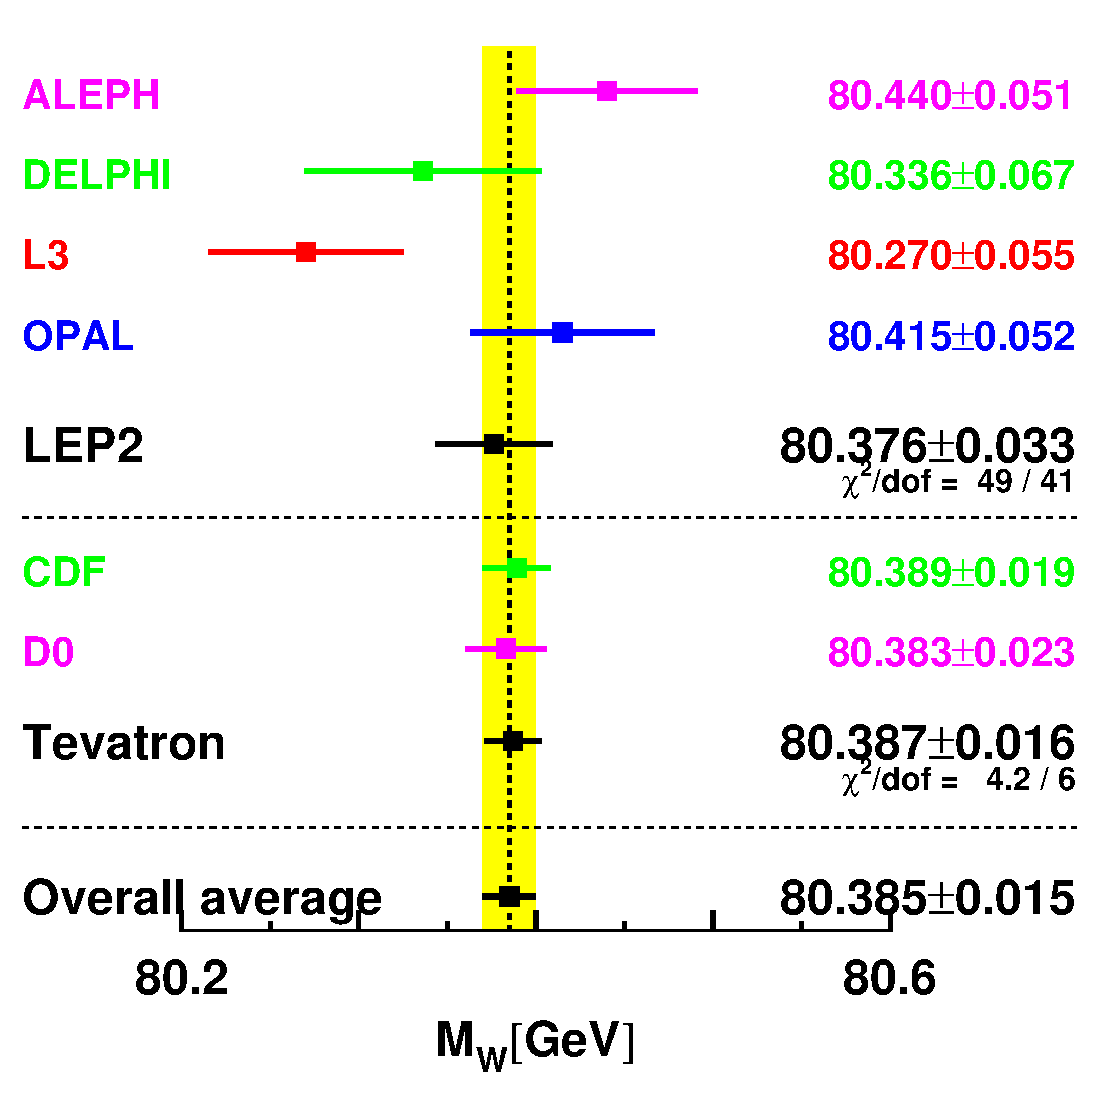
\includegraphics[width=.45\textwidth]{figures/theory/wmass_pdg.eps}
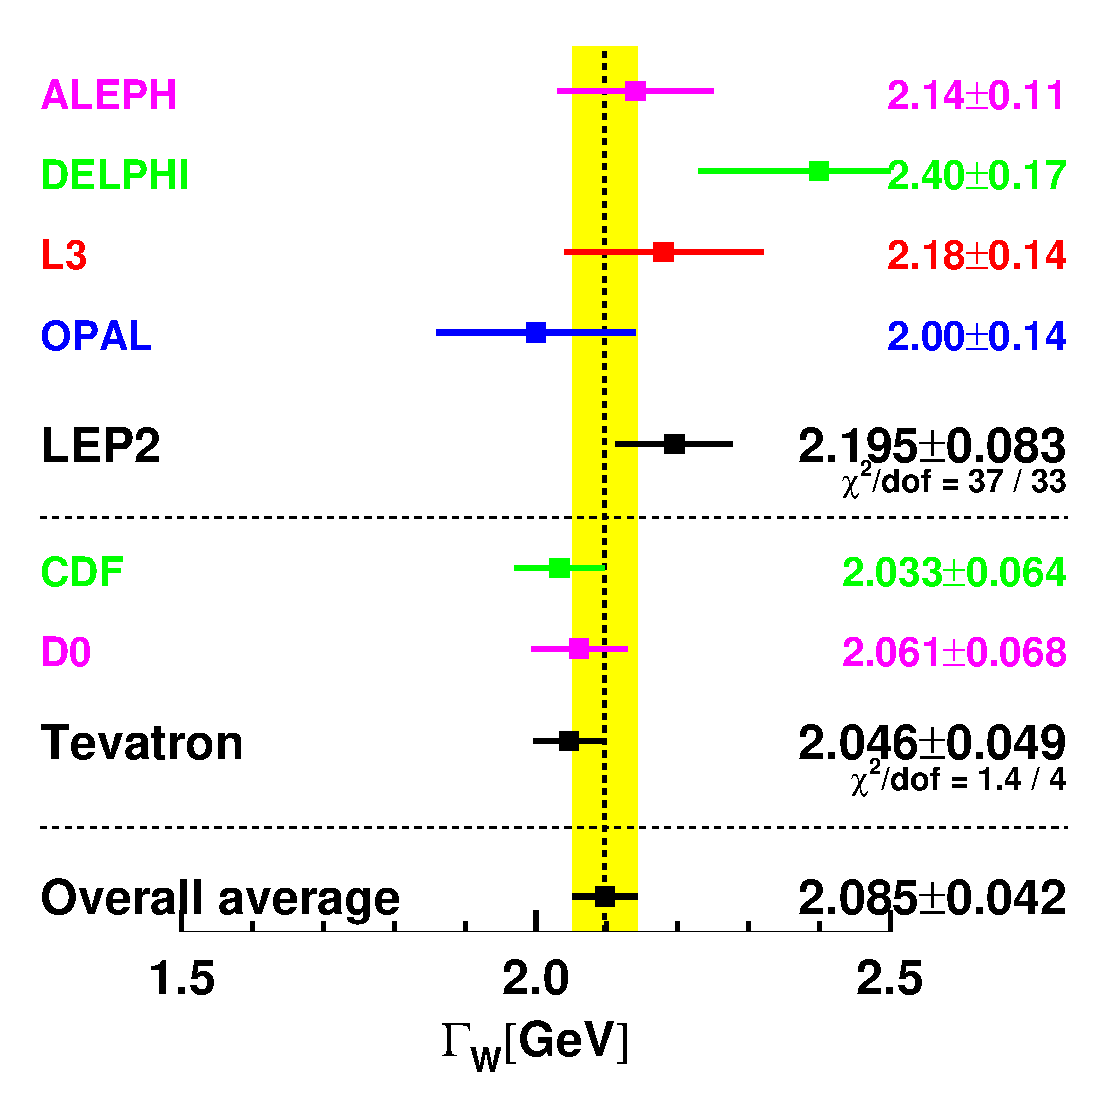
\includegraphics[width=.45\textwidth]{figures/theory/wwidth_pdg.eps}
\caption{Summary of \dubya~mass (left) and width (right) measurements
as performed at LEP and the Tevatron~\cite{PDG:2014}.}
\label{fig:theory_w_pdg}
\end{figure}


While the fundamental parameters of the EW theory are related to each other
by relations like those above, they are not determined \emph{a priori} 
and so must be first determined from experiment.
Of primary interest to the topic of this thesis 
are the measured parameters related to the behavior and properties
of the \dubya~and Higgs bosons.
The \dubya~was first discovered in 1983 via $p\overline{p}$ collisions
at the SPS by looking at its decay to an electron %abbreviation?
and electron neutrino \cite{ARNISON1983103}.
Its mass has been measured in $p\overline{p}$ collisions at the Tevatron
and in $e^{+}e^{-}$ collisions at LEP to give a world 
average of $80.385 \pm 0.015\GeV$~\cite{PDG:2014}.
A summary of the \dubya~mass measurements is shown on 
the right of \fig\ref{fig:theory_w_pdg}.
The width assuming a Breit-Wigner distribution has also been measured 
at LEP and the Tevatron as seen in the right of \fig\ref{fig:theory_w_pdg}
with an average value of $2.085\pm0.042\GeV$ \cite{PDG:2014}.
Roughly 1/3 of of the time the \dubya~decays approximately 
evenly into each of the three lepton generations,
as expected from the shared coupling of \eqn\eqref{eq:couplings_wleptons}
(ignoring kinematics).
The leptonic decays of the \dubya~result in a charged lepton 
with the same charge as the parent \dubya~(as dictated by charge conservation)
and a neutrino (or anti-neutrino if the parent \dubya~has negative charge),
as indicated in the top of \fig\ref{fig:feyn_wcoupling}.
The \dubya~decays into quarks the remaining 2/3 of the time with a positively
(negatively) charged \dubya~decaying into a up-type quark (anti-quark) 
and down-type anti-quark (quark),
like in the bottom of \fig\ref{fig:feyn_wcoupling}.
The measured branching fractions for the \dubya~are 
summarized in \tab\ref{tab:theory_wdecay}.

\begin{table}[ht]
\centering
\begin{tabular}{l|c}
Decay Mode &  Branching Fraction [\%]\\
\hline
$e^+\nu_e$ ($e^-\overline{\nu}_e$) & $10.71 \pm 0.16$ \\
$\mu^+\nu_{\mu}$ ($\mu^-\overline{\nu}_{\mu}$) & $10.63 \pm 0.15$\\
$\tau^+\nu_{\tau}$ ($\tau^-\overline{\nu}_{\tau}$) & $11.38 \pm 0.21$\\
Quarks & $67.41 \pm 0.27$\\
\end{tabular}
\caption{Measured branching fractions of the $\dubya^+$ ($\dubya^-$)~boson 
as reported by the Particle Data Group \cite{PDG:2014}.  The $W$ decays
to quarks result in hadronic states which in general prohibit
one from determining the specific $W$ final state. Thus, only 
an inclusive branching fraction is listed for the decay to quarks.}
\label{tab:theory_wdecay}
\end{table}


%The cross-section of the production of the \dubya~at colliders
%depends on the initial state (i.e. $pp$ vs $p\overline{p}$) and on the
%collision energy. 
%The cross-section times branching fraction to leptons 
%has been measured thoroughly, with separate measurements performed
%at RHIC~\cite{PhysRevLett.106.062001};
%the SPS~\cite{Albajar1987271,Alitti1992365};
%the Tevatron~\cite{0954-3899-34-12-001,D0-4403-CONF};
%and most recently at the LHC 
%at 7~\TeV~\cite{PhysRevD.85.072004,Chatrchyan:1370079}, 
%8~\TeV~\cite{PhysRevLett.112.191802}, 
%and 13~\TeV~\cite{ATLAS-CONF-2015-039,CMS-PAS-SMP-15-004}. 
%A summary of these measurements is shown in 
%\fig\ref{fig:theory_wxsec} which reveals them to be in good agreement with 
%the predictions.

%\begin{figure}[ht]
%\centering
%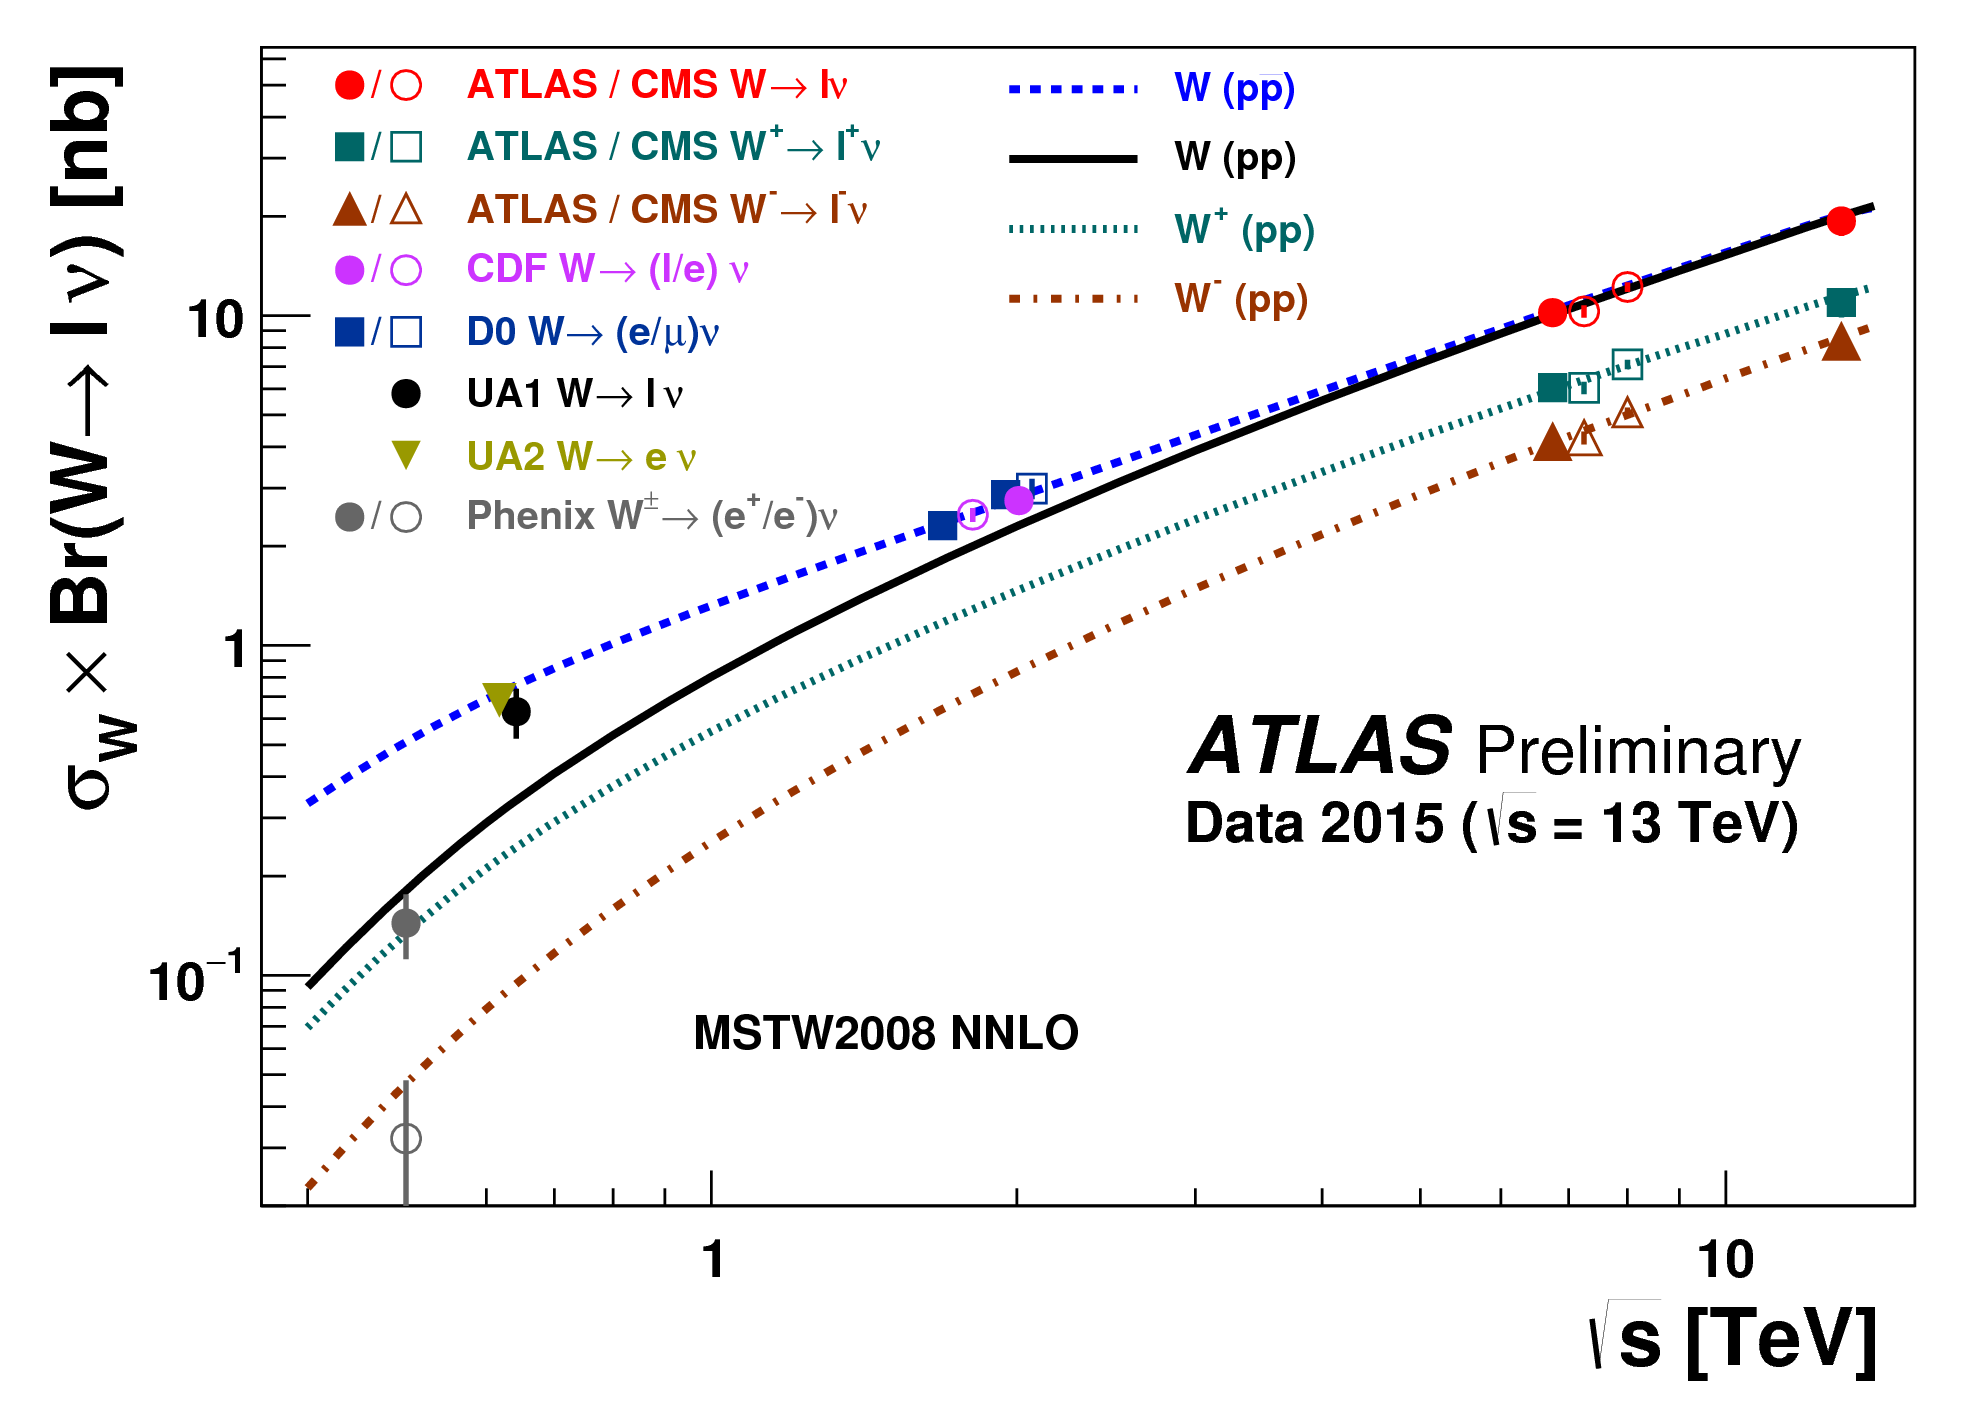
\includegraphics[width=.8\textwidth]{figures/theory/wxsec.png}
%\caption{Summary of $W\rightarrow l\nu$ cross-section measurements as 
%a function of center-of-mass energy, $\sqrt{s}$. 
%Next-to-next-to-leading-order (NNLO) theoretical
%predictions are shown for both $pp$ and 
%$p\overline{p}$ collisions and for $pp$ collisions when split by charge.
%Experimental measurements are overlayed and taken from measurements
%at the SPS, RHIC, the Tevatron, and the LHC.  The plot is taken
%from the ATLAS publication of $W$ and $Z$ cross-section measurements
%at the LHC \cite{ATLAS-CONF-2015-039}.  }
%\label{fig:theory_wxsec}
%\end{figure}

The Higgs boson was discovered in 2012 at the LHC
jointly by ATLAS \cite{Aad20121} and CMS \cite{Chatrchyan:2012xdj}.
Combined measurements of the mass between the two experiments 
show the current value of the Higgs mass to be 
$m_H = 125.09 \pm 0.21 (\textrm{Stat.}) \pm 0.11 (\textrm{Syst.})\GeV$
\cite{Aad:2015zhl} as seen in \fig\ref{fig:higgs_mass}.
Detailed studies of the spin \cite{Aad2013120,Khachatryan:2014kca},
width \cite{Aad:2015xua,Khachatryan:2014iha},
and couplings \cite{ATLAS-CONF-2015-044} are all consistent
with the Higgs boson of the SM.

\begin{figure}
\centering
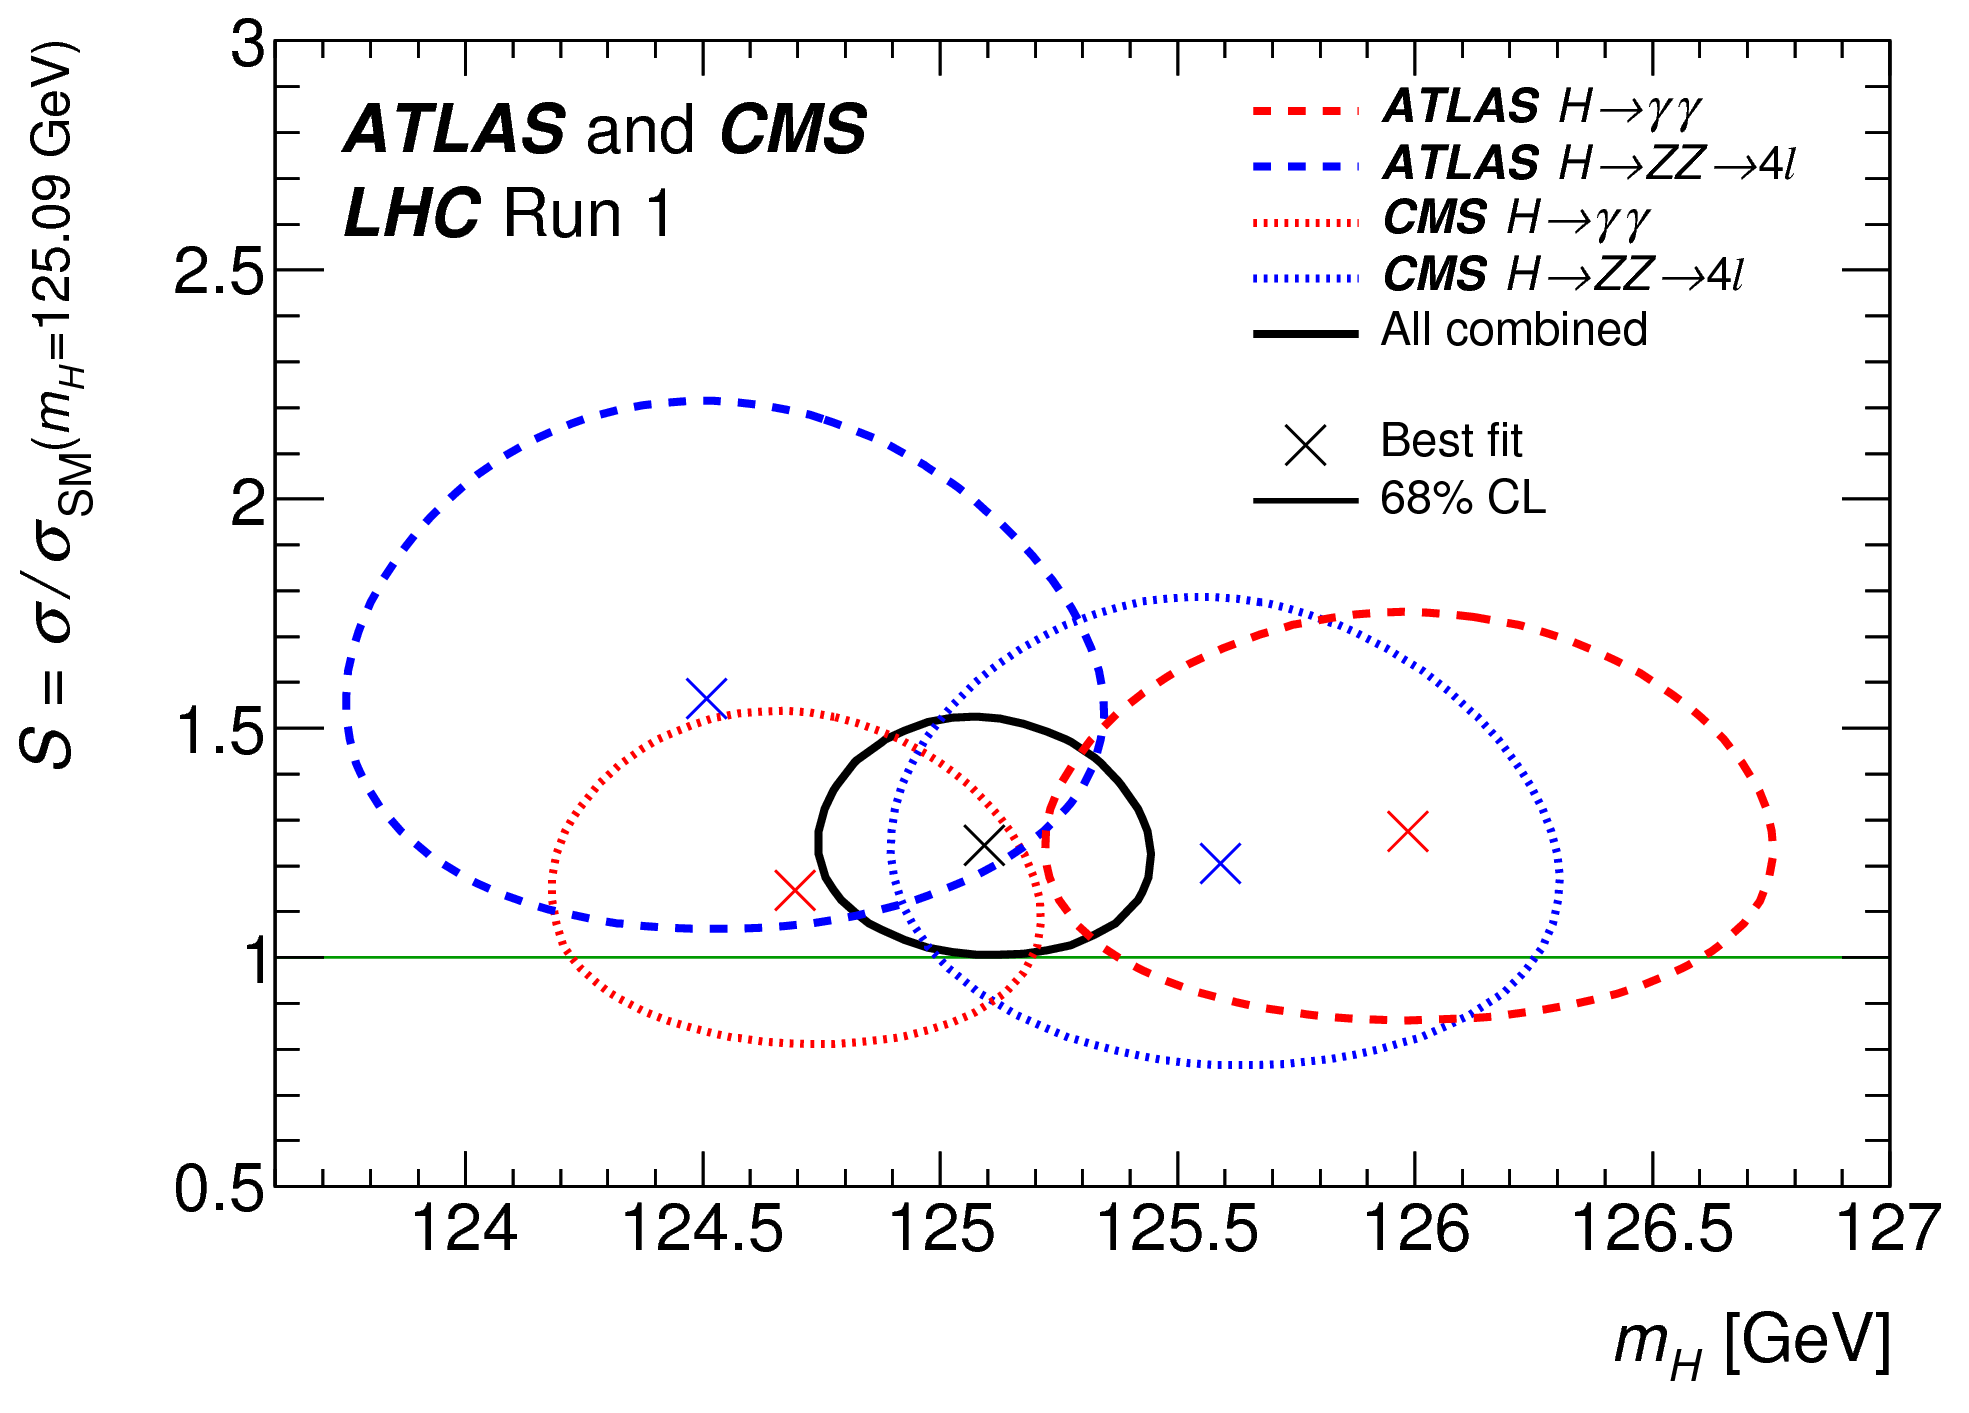
\includegraphics[width=.8\textwidth]{figures/theory/higgs_mass.png}
\caption{Combined ATLAS and CMS 
measurements of Higgs signal strength
vs mass in $H\rightarrow \gamma \gamma$ and $H\rightarrow ZZ\rightarrow 4l$
channels with 68\%CL likelihood curves \cite{Aad:2015zhl}.}
\label{fig:higgs_mass}
\end{figure}

\section{$WWW$ Production}

\unitlength = 0.6mm %necessary for feynmp
\begin{figure}[ht]
\centering
\vspace{5 mm}
\begin{fmffile}{feynwwwprod1}
		\begin{fmfgraph*}(80,50)
			\fmfleft{i1,i2}
			\fmfright{o1,o2,o3}

			\fmf{fermion}{i1,v1}
			\fmf{fermion}{v1,i2}
			\fmf{photon}{v1,v2}
			\fmf{photon}{v2,o1}
			\fmf{photon}{v2,o2}
			\fmf{photon}{v2,o3}
		\end{fmfgraph*}
\end{fmffile}
\hspace{6 mm}
\begin{fmffile}{feynwwwprod2}
		\begin{fmfgraph*}(80,50)
			\fmfleft{i1,i2}
			\fmfright{o1,o2,o3}

			\fmf{fermion}{i1,v1}
			\fmf{fermion}{v1,i2}
			\fmf{photon}{v1,v2}
			\fmf{photon}{v2,o1}
			\fmf{dashes,label=$H^0$}{v2,v3}
			\fmf{photon}{v3,o2}
			\fmf{photon}{v3,o3}
		\end{fmfgraph*}
\end{fmffile}

\vspace{6 mm}
\begin{fmffile}{feynwwwprod3}
		\begin{fmfgraph*}(80,50)
			\fmfleft{i1,i2}
			\fmfright{o1,o2,o3}

			\fmf{fermion}{i1,v1}
			\fmf{fermion}{v1,v2}
			\fmf{fermion}{v2,v3}
			\fmf{fermion}{v3,i2}
			\fmf{photon}{v1,o1}
			\fmf{photon}{v2,o2}
			\fmf{photon}{v3,o3}
		\end{fmfgraph*}
\end{fmffile}
\hspace{6 mm}
\begin{fmffile}{feynwwwprod4}
		\begin{fmfgraph*}(80,50)
			\fmfleft{i1,i2}
			\fmfright{o1,o2,o3}
			\fmf{fermion}{i1,v1}
			\fmf{fermion}{v1,v2}
			\fmf{fermion}{v2,i2}
			\fmf{photon,label=$Z/\gamma^{*}$}{v2,v3}
			\fmf{photon}{v1,o1}
			\fmf{photon}{v3,o2}
			\fmf{photon}{v3,o3}
		\end{fmfgraph*}
\end{fmffile}
\vspace{2 mm}
\caption{The tree level Feynman diagrams 
for $WWW$ production. The incoming fermion
lines in each diagram consist of an
up-type quark (anti-quark) and down-type anti-quark (quark). Unless
otherwise specified, the curved lines correspond to $W$ bosons.}
\label{fig:theory_feynman_www}
\end{figure}

In this thesis, we are interested in the inclusive production of three
$W$ bosons from proton-proton collisions:
$pp\rightarrow\- \Wp\Wp\Wm+X$ and $pp\rightarrow \Wp\Wm\Wm\allowbreak +X$, 
where $X$ is intended to refer to the fact that no requirements are 
placed on additional particles produced in the hard interaction.
This is sensitive both
to the $WWWW$ coupling (non-resonant production) 
and to associated Higgs production \footnote{Associated Higgs production involves
the radiation of a Higgs boson off another particle (in this case a $W$ boson). It 
is sometimes referred to as ``Higgsstrahlung'', by analogy 
with electron Bremsstrahlung where an electron radiates a photon.} where 
the Higgs decays to two
$W$ bosons (resonant production). 
The relevant
tree-level Feynman diagrams for this production process are shown in 
\fig\ref{fig:theory_feynman_www}.
The Higgs decay results in one $W$ boson being produced off-shell,
$H\rightarrow WW^*$, making this the leading contribution to off-shell
production.  
The resonance from the Higgs can clearly be seen from the 
distribution of $m_{\Wp\Wm}$ taken from the simulation of production \www~events
in \fig\ref{fig:mww_higgs}.

%It would be nice to show a plot of the Higgs stuff. maybe I can
%steal this and make my own later...
\begin{figure}[ht]
\centering
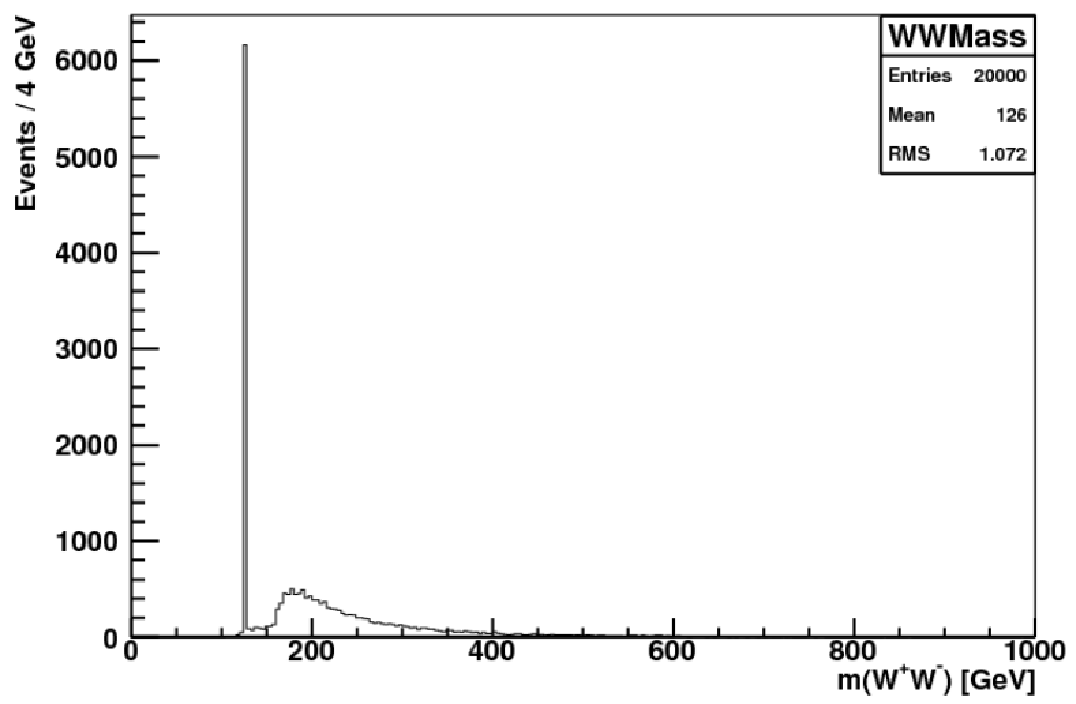
\includegraphics[width=0.5\columnwidth]{figures/2l2j/mWW-parton.pdf}
\caption{ Invariant mass distribution of two opposite-sign $W$ bosons 
in \www events generated with VBFNLO at LO. The Higgs mass peak is clearly 
visible at 126~GeV. (make a better plot)}
\label{fig:mww_higgs}
\end{figure}




The cross-section for this process can be computed at 
next-to-leading-order (NLO) in QCD
( $O(\alpha_s^2)$ in perturbation theory (?) ). 
(Mention more details of how this is computed like PDFs,
hadronization, interaction, radiation, decays. Use one of the 
Feynman diagrams)
Using 
the \madgraph~generator finds an inclusive cross-section of 
\begin{equation}
\sigma(pp\rightarrow WWW + X) = 241.47 \pm 0.13~\textrm{fb}
\label{eq:www_total_xsec}
\end{equation}
where the uncertainty is purely statistical.
The contribution from resonant production is computed separately
and found to make up about 64\% of the 
total inclusive cross-section.
More details on the determination of the signal cross-section, uncertainties,
and kinematics are presented in \sec\ref{sec:signal}.

\begin{figure}
\centering
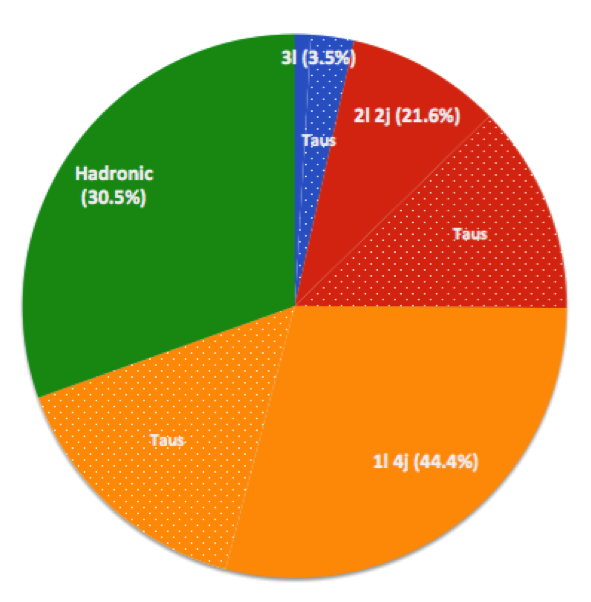
\includegraphics[scale=.8]{figures/branching_fractions.png}
\caption{Pie chart showing the different decay modes contributing 
to the total \xsec for the \www~process. 
The dotted areas indicate the portion of each decay 
mode which is due to the production of tau leptons.}
\label{fig:branching_fractions}
\end{figure}

Due to the short lifetime of the $W$ boson, each of the $W$ bosons
in the $WWW$ process will decay before reaching the detector.
This results in a measurable final state for the $WWW$ production 
process that includes some combination of leptons 
and quarks (manifested as jets).  The branching fractions for 
the $WWW$ process can be determined from the individual $W$ branching fractions
listed in \tab\ref{tab:theory_wdecay}.  The expected $WWW$ branching
fractions are thus summarized in the pie chart in \fig\ref{fig:branching_fractions}.
For this thesis, we are primarily interested in the final state
where each $W$ boson decays leptonically (the fully-leptonic final state) 
which has the smallest branching fraction at roughly 3.5\%.
In fact, since the $\tau$ leptons are also unstable, we choose to 
omit $W$ decays to $\tau$ leptons from our fully-leptonic
definition as well. This further reduces the fully-leptonic 
branching fraction to 0.97\%.  While small, this fully-leptonic final state
should have smaller backgrounds to the signal than the other 
decay channels, making it one of the most sensitive channels for studying
this process. The branching fraction when one $W$ boson is allowed
to decay hadronically is considerably larger, at 21.6\% (or
9.2\% when excluding decays to $\tau$ leptons). This is 
referred to as the semi-leptonic decay channel. The presence
of the two leptons from the other two $W$ decays still allows
for background discrimination, though not as much as in the fully-leptonic
channel. As a result, this channel has also been studied, though it 
is not the focus of this thesis. The remaining channels have
not been studied. The combination of the fully-leptonic
and semi-leptonic channels is presented in \sec\ref{sec:measurement}.



\section{Effective Field Theory}

The lagrangian of the SM, summarized by 
\eqn\eqref{eq:lagrangian_sm},~\eqref{eq:lagrangian_qcd},
~\eqref{eq:lagrangian_ew}, and~\eqref{eq:lagrangian_ewsb}
has so far been very successful. 
But, as we continue to probe higher energy scales, 
there is reason to believe that the SM's luck will run out.
If history is any guide, the SM is simply
an approximation of a larger theory whose details are not relevant
relevant at current energies.
Indeed, the SM leaves important questions unanswered (for example, 
the hierarchy problem) that could be explained
by the observation of some new high energy phenomena.  %more detail

This idea of the SM as an approximate theory
can be made explicit 
using an Effective Field Theory (EFT) \cite{Pich:1998xt}
approach which includes new terms in the lagrangian, in addition to the SM.
As a function of the energy, these terms start small 
but become increasingly important at higher and higher energies.
In general, the new EFT terms might look like this:
\begin{equation}
\curlyl_{\textrm{EFT}} = \curlyl_{\textrm{SM}} + \sum_{n=5}^{\infty} \sum_i \frac{c_{n,i}}{\Lambda^{n-4}} \curlyo_{n,i}
\end{equation}
where $\Lambda$ is some new energy scale relevant to the new
physics we seek to describe and the $c_{n,i}$ are dimensionless
couplings.  While the operators of the SM have mass dimension 4, the EFT 
operators, $\curlyo_{n,i}$, have a mass dimension
$n>4$ which describe the new interactions between the SM fields at low energy
due to the new physics model.
The sum over $i$ is simply to indicate that there are in general multiple 
possible new operators for a given mass dimension.
These EFT operators come from ``integrating out'' the high energy interactions
between the SM fields and the fields in the new physics model,
leaving behind contact interactions between the SM fields and factors
of $\Lambda^{n-4}$ in the denominator.
These factors of $\Lambda$ suppress the new terms
with respect to the SM, with the suppression becoming stronger as $n$ grows.
Thus, only the first terms in the summation
over $n$ are important at low energy.

The list of possible gauge-invariant EFT operators to 
consider is long \cite{Hagiwara:1993ck,Buchmuller:1985jz,Eboli:2006wa}
One way to shorten the list is to impose certain symmetries. 
Enforcing the conservation
of baryon and lepton number restricts 
us to only even values of $n$:
\begin{equation}
\curlyl_{\textrm{EFT}} = \curlyl_{\textrm{SM}} + \sum_i \frac{c_{6,i}}{\Lambda^2} \curlyo_{6,i} + \sum_j \frac{c_{8,j}}{\Lambda^4} \curlyo_{8,j} + \dots
\label{eq:lagrangian_eft}
\end{equation}
where we have truncated the series at $n=8$ since these
these higher order terms are small.
The leading $n=6$ terms predict new anomalous triple and quartic 
gauge coupling (aTGC and aQGC) interactions while the sub-leading $n=8$ terms
predict only new aQGC interactions. 
Predictions of aTGC interactions have been studied in detail at 
LEP, the Tevatron, and the LHC  with no luck \cite{PDG:2014}.
But there is still hope!
It could be that new physics is suppressed in aTGC interactions
but not in aQGC interactions. \footnote{For instance, the aTGC interactions
could first appear at the one loop level while the aQGC 
interactions appear at tree level.}
Then the new physics might first appear at $n=8$, where only aQGC interactions
occur.



%\subsection{Anomalous Quartic Gauge Couplings}

In a linear EFT model where the Higgs field is indeed the mechanism for EWSB, 
the possible $n=8$ operators 
in \eqn\eqref{eq:lagrangian_eft} can
be split into three categories: those containing covariant derivatives,
as in \eqn\eqref{eq:ew_covariant_derivative}, of the Higgs field, $\phi$; 
those containing covariant derivatives of the Higgs field and 
the field strength tensors, as 
in \eqn\eqref{eq:wfieldstrength} and \eqref{eq:bfieldstrength};
or those containing only field strength tensors \cite{Eboli:2006wa,Eboli:2003nq}. 
All of these operators preserve CP symmetry.
In this thesis, we are
interested only in the first category, which is limited to just two operators:
\begin{align}
\curlyo_{S,0} =& \Big[(D_{\mu}\phi)^{\dagger} D_{\nu} \phi\Big] \times \Big[(D^{\mu} \phi)^{\dagger} D^{\nu} \phi \Big] \\
\curlyo_{S,1} =& \Big[(D_{\mu}\phi)^{\dagger} D^{\mu} \phi\Big] \times \Big[(D_{\nu} \phi)^{\dagger} D^{\nu} \phi \Big]
\end{align}
which could come from integrating out some new 
vector gauge boson resonance coupling to the EW gauge bosons \cite{Baak:2013fwa}.
Plugging these into \eqn\eqref{eq:lagrangian_eft} (and dropping all other terms
besides the SM), we get
\begin{equation}
\begin{aligned}
\curlyl_{\textrm{EFT}} = \curlyl_{\textrm{SM}} +&
\frac{f_{S,0}}{\Lambda^4}\Big[(D_{\mu}\phi)^{\dagger} D_{\nu} \phi\Big] \times \Big[(D^{\mu} \phi)^{\dagger} D^{\nu} \phi \Big] \\
+& \frac{f_{S,1}}{\Lambda^4}\Big[(D_{\mu}\phi)^{\dagger} D^{\mu} \phi\Big] \times \Big[(D_{\nu} \phi)^{\dagger} D^{\nu} \phi \Big]
\end{aligned}
\label{eq:lagrangian_aqgc}
\end{equation}
where we have introduced the new arbitrary couplings $f_{S,0}$ and $f_{S,1}$.
Expanding this out we get...
These modify the SM QGC interactions of \eqn\eqref{eq:lagrangian_qgc}
and \fig\ref{fig:theory_feynman_couplings_qgc}
to produce new aQGC interactions $W^+W^-W^+W^-$, $W^+W^-ZZ$, and $ZZZZ$
that do not depend on the gauge boson momenta (do I care?).
In this thesis, we are interested only in the aQGC
interaction term involving $W^+W^-W^+W^-$, which predicts  
a new tree level diagram for the $WWW$ production process similar to the SM QGC
production of this process in \fig\ref{fig:theory_feynman_couplings_qgc}.
If real, such a modification would enhance the predicted 
cross-section in \eqn\eqref{eq:www_total_xsec}.

By definition, the EFT approach is expected to break for energies
greater than $\Lambda$. Thus the issue arises of what energy 
$\Lambda$ corresponds to.

Unitarity...
not UV complete
effective lagrangian (could be used elsewhere to refer to the eft lagrangian)
the effect from unitarity violation typically sets in earlier due to the higher exponent in Lambda in the denominator. 

Unitarity violation is somehow related to how we can choose Lambda


\section{Status of QGC Measurements and aQGC Limits}
A variety of measurements sensitive QGC interactions have been
performed at colliders. In particular, measurements sensitive
to $WW\gamma\gamma$ have been performed 
at LEP \cite{Abdallah:2003xn,PhysRevD.70.032005}, 
the Tevatron \cite{PhysRevD.88.012005}, %is this really the only Tevatron measurement??
and the LHC \cite{PhysRevLett.115.031802,PhysRevD.90.032008,Chatrchyan:2013akv}; 
%mention how they were probed?
to $WWZ\gamma$ at LEP~\cite{Achard:2001eg,Abbiendi:1999aa,Abbiendi:2003jh}
and at the LHC~\cite{PhysRevD.90.032008};
to $ZZ\gamma\gamma$ at LEP \cite{Achard:2002iz,PhysRevD.70.032005}; 
and to $WWWW$ at the LHC \cite{PhysRevLett.113.141803,PhysRevLett.114.051801}. 
%Typically, these studies are performed
%by looking at x final state (more detail). 
%The first measurements sensitive to the $WWWW$ vertex focused on 
%same-sign $WW$ vector boson scattering because...

%material on limits?

%summary plots? maybe from PDG?

More details?


